% Seção 5: Pesquisa Autoral
\section{Pesquisa Autoral}
\begin{frame}{Disseminação de Eventos Críticos por VANETS\footcite{Andrade2021a,Andrade2021b}}
    \begin{columns}
        \begin{column}{0.65\textwidth}
            \begin{figure}
                \centering
                \subfloat{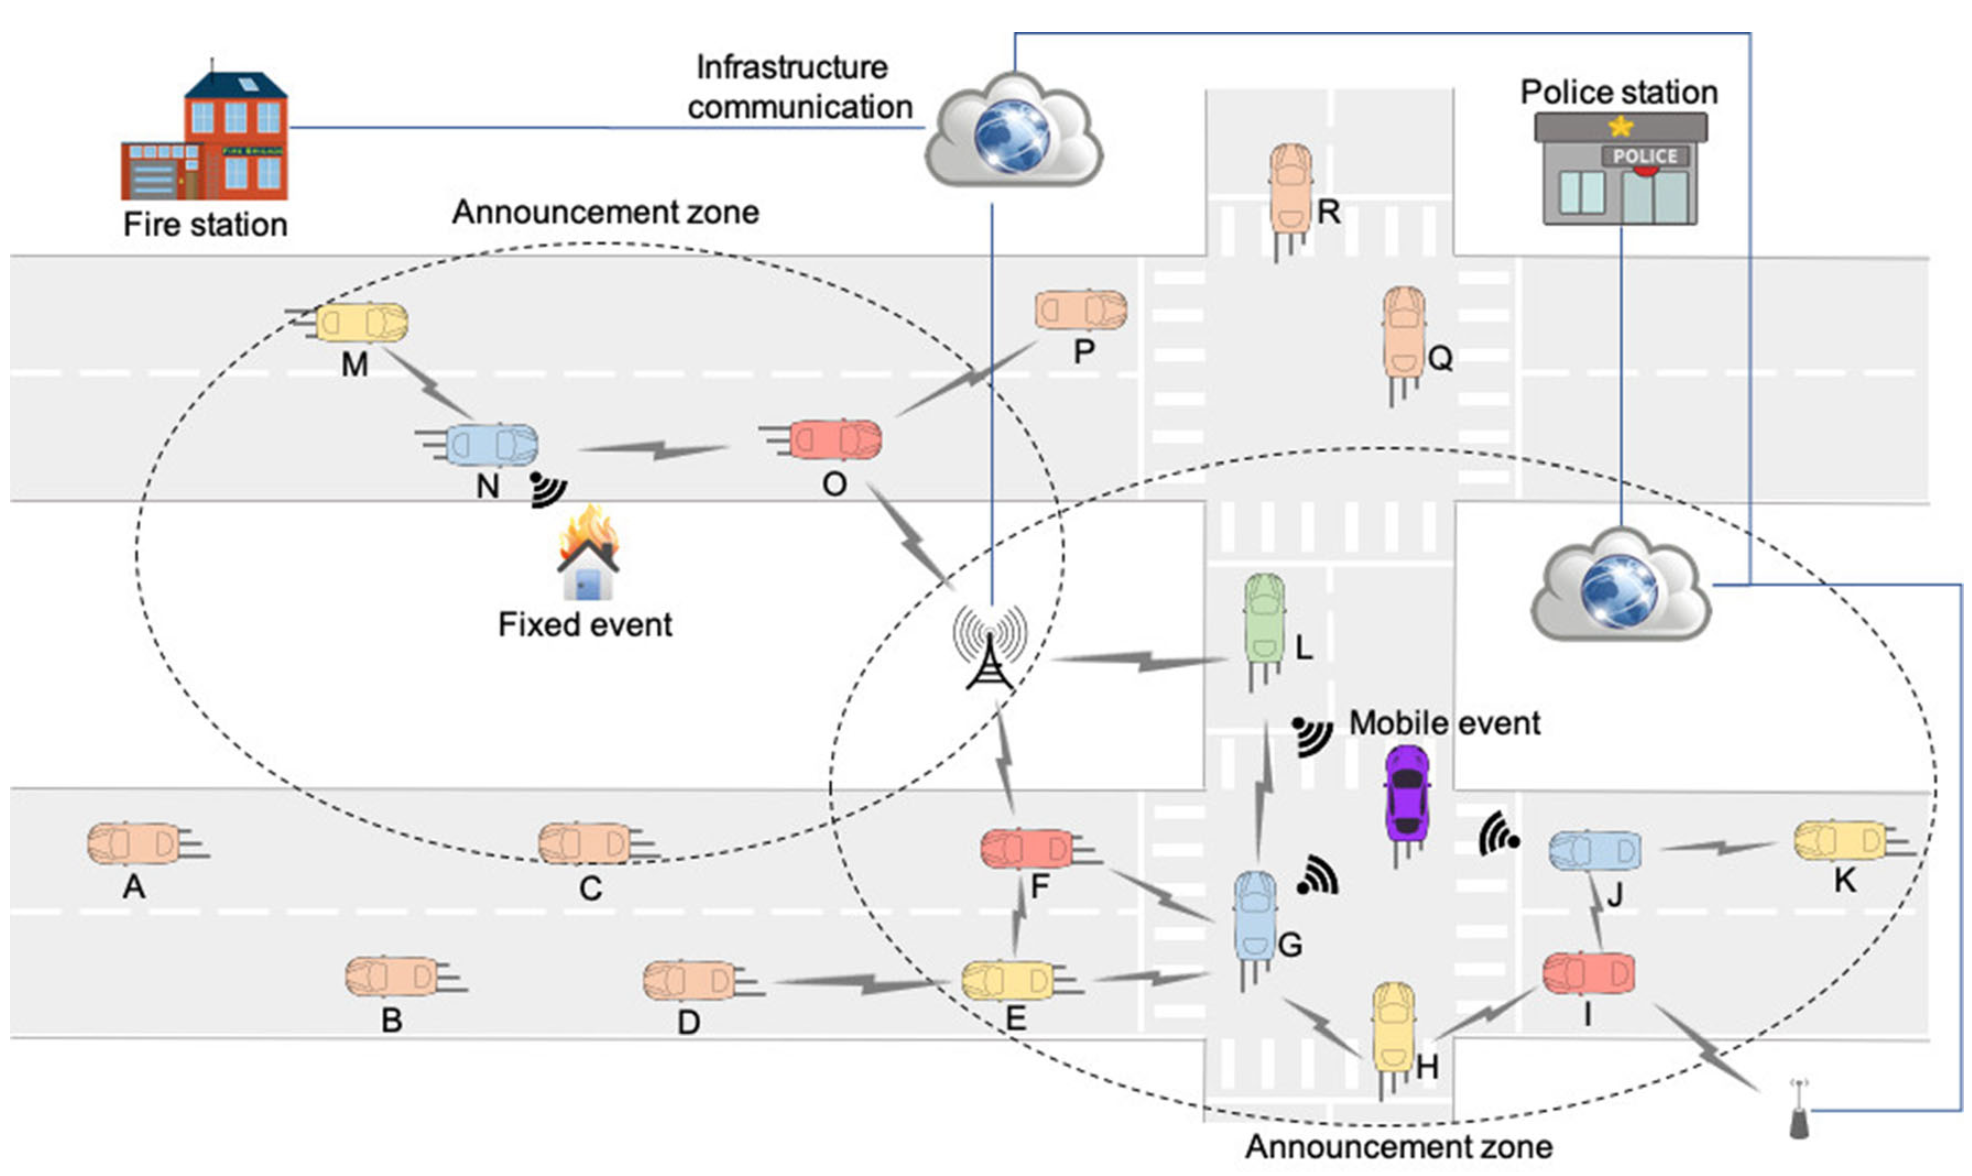
\includegraphics[width=0.85\linewidth]{figs/minuet_cenario.png}}\quad
                \subfloat{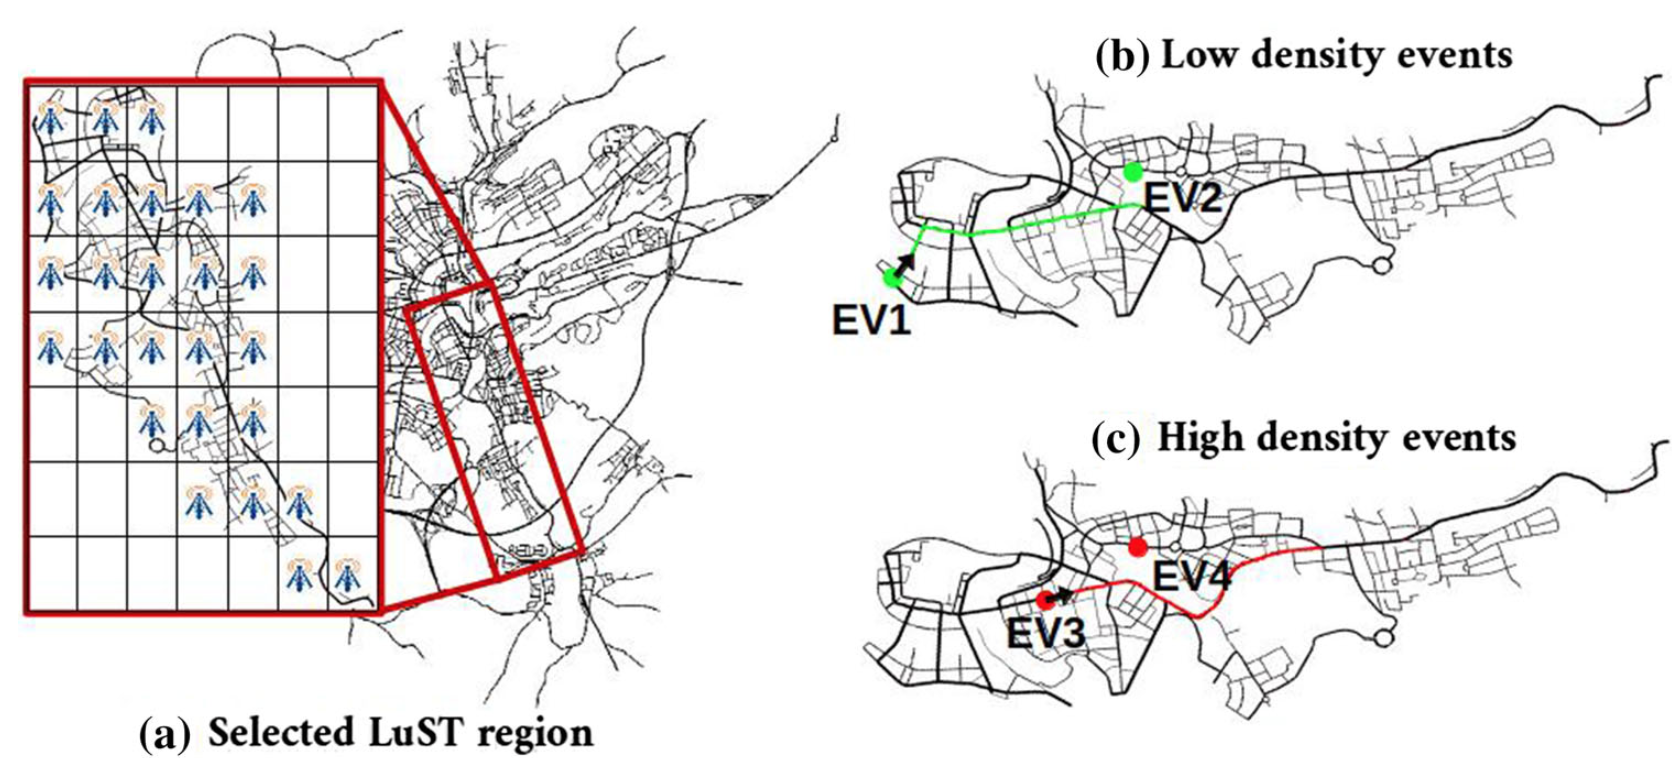
\includegraphics[width=0.75\linewidth]{figs/minuet_lust.png}}
                \caption{Topologia e cenário}
                \label{fig:enter-label}
            \end{figure}    
        \end{column}
        \begin{column}{0.35\textwidth}
            \begin{figure}
                \centering
                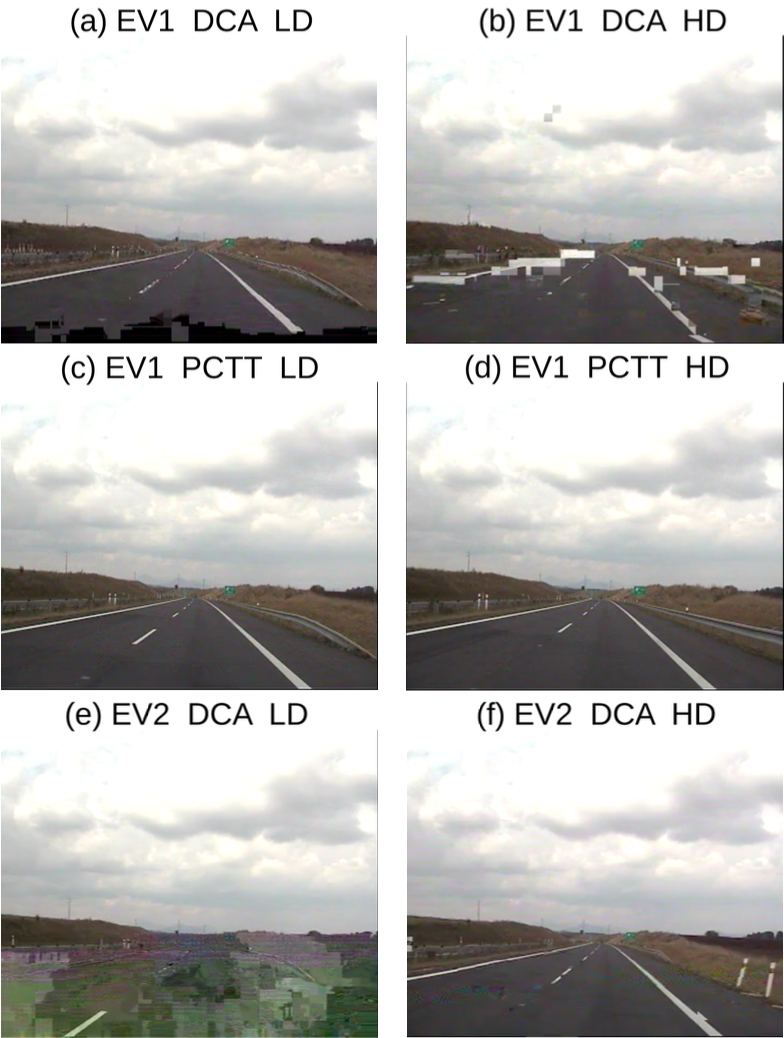
\includegraphics[width=0.9\linewidth]{figs/minuet_video.png}
                \caption{Resultados}
                \label{fig:enter-label}
            \end{figure}
        \end{column}
    \end{columns}
\end{frame}

\begin{frame}{Orquestração e Gerência de \textit{Cloud-Network Slices}\footcite{Rocha2022}}
    \begin{columns}
        \begin{column}{0.5\linewidth}
            \begin{figure}
                \centering
                \subfloat{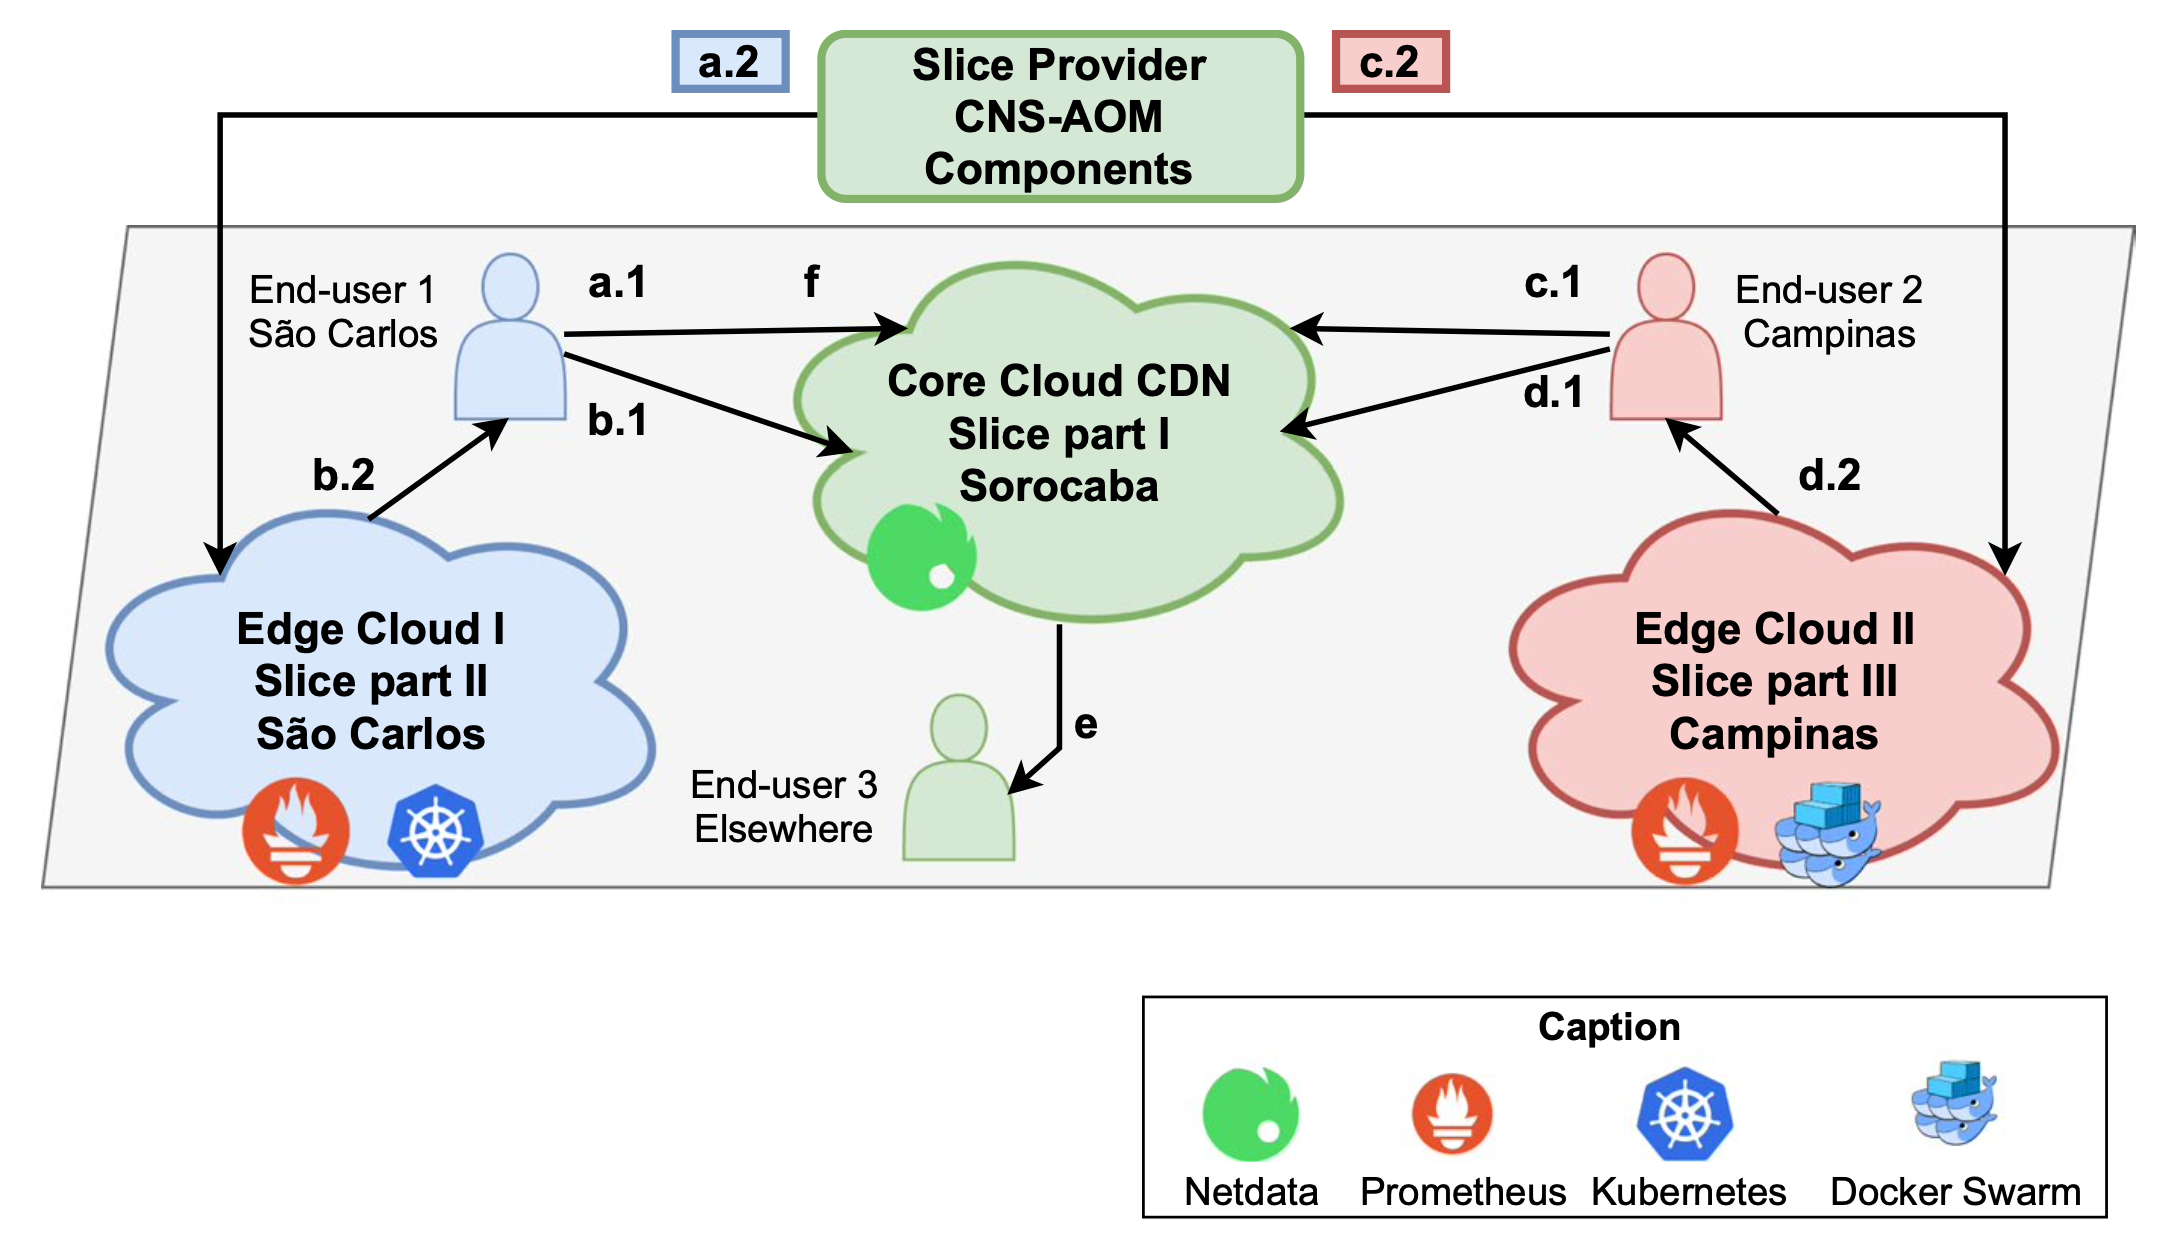
\includegraphics[width=0.9\linewidth]{figs/SEA_POC_VoD.png}}\quad
                \subfloat{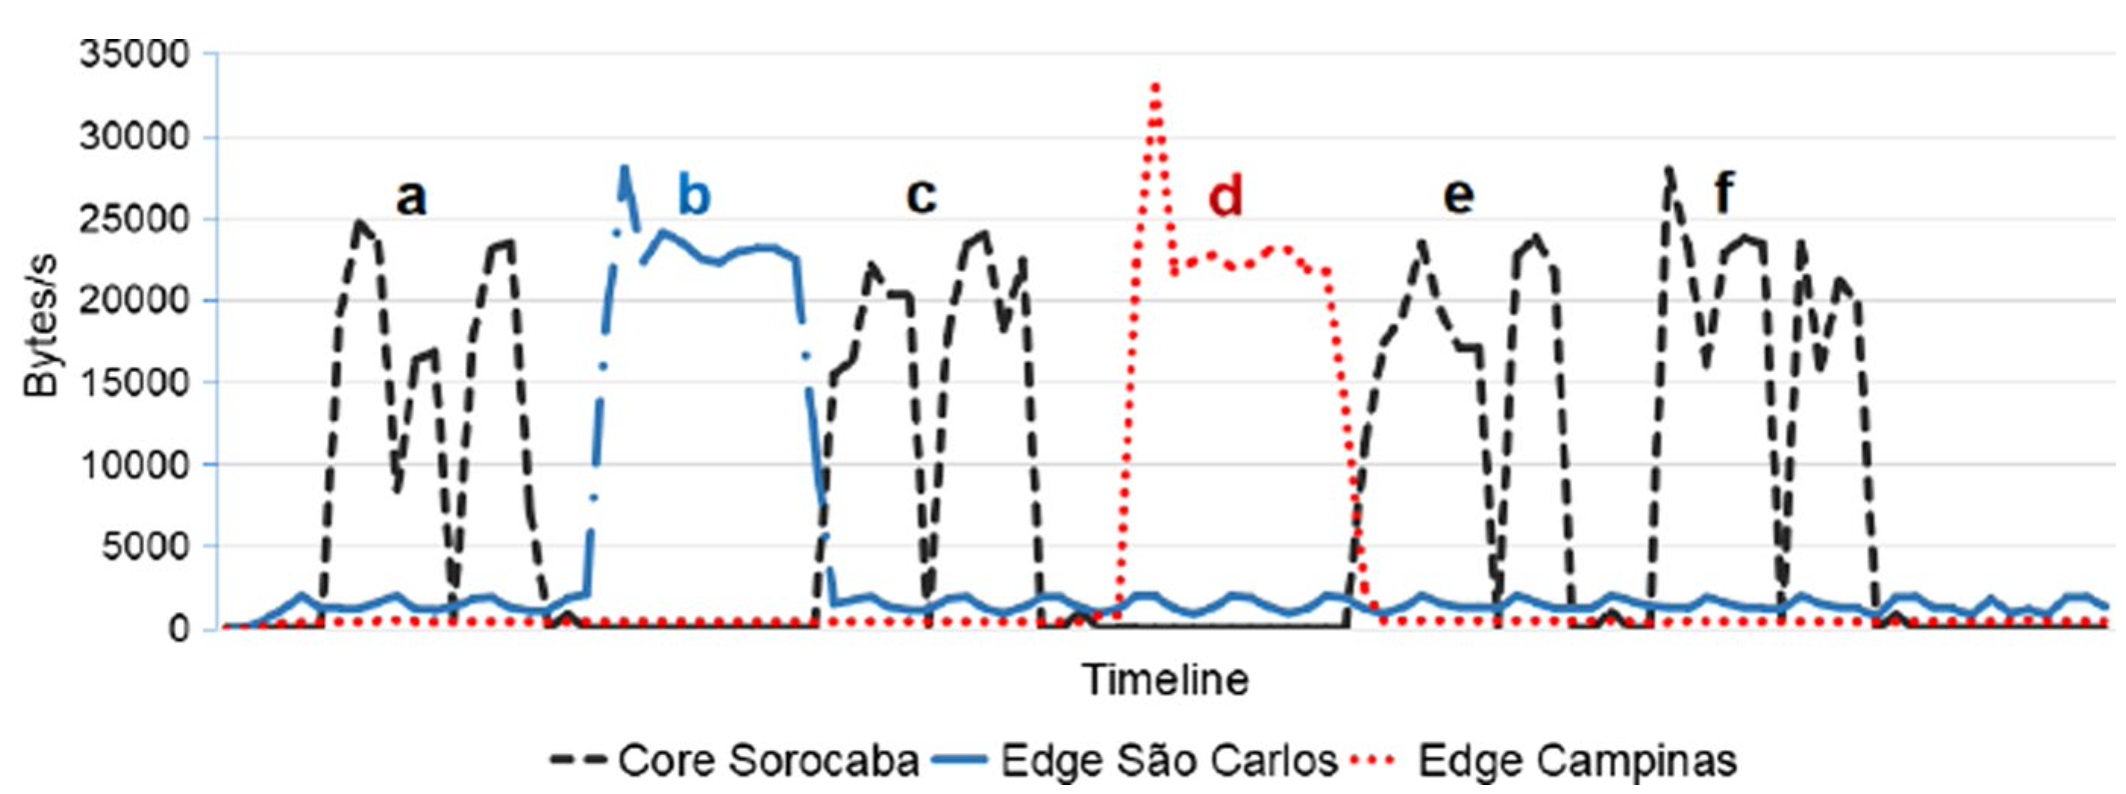
\includegraphics[width=0.9\linewidth]{figs/SEA_Plot_VoD.png}}
                \caption{PoC VoD}
            \end{figure}            
        \end{column}
        \begin{column}{0.5\linewidth}
            \begin{figure}
                \centering
                \subfloat{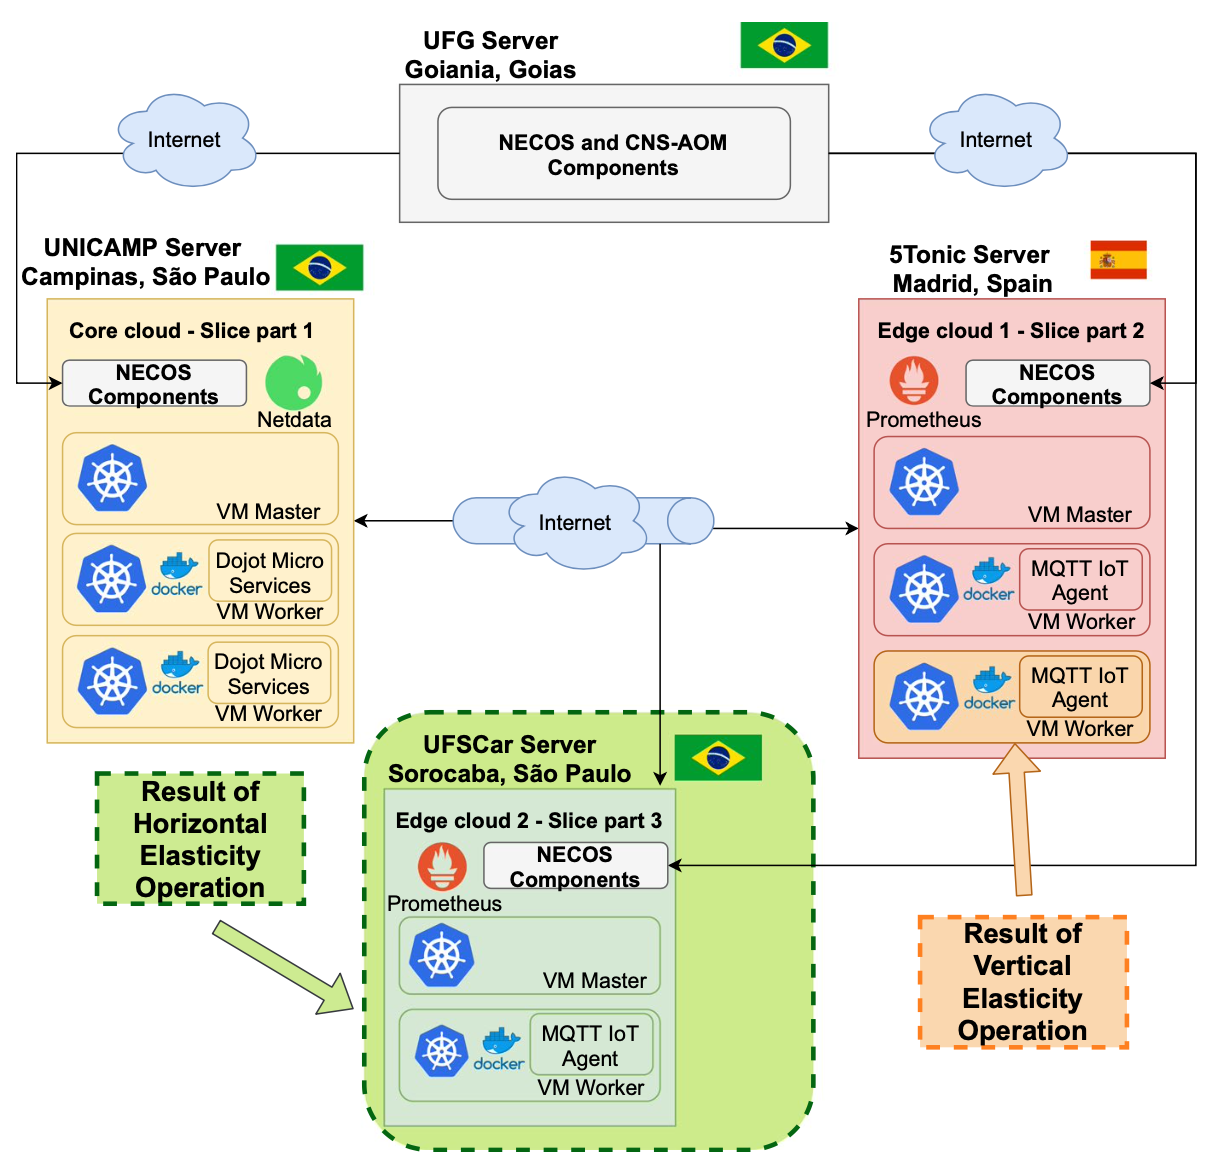
\includegraphics[width=0.8\linewidth]{figs/SEA_POC_IoT.png}}\quad
                \subfloat{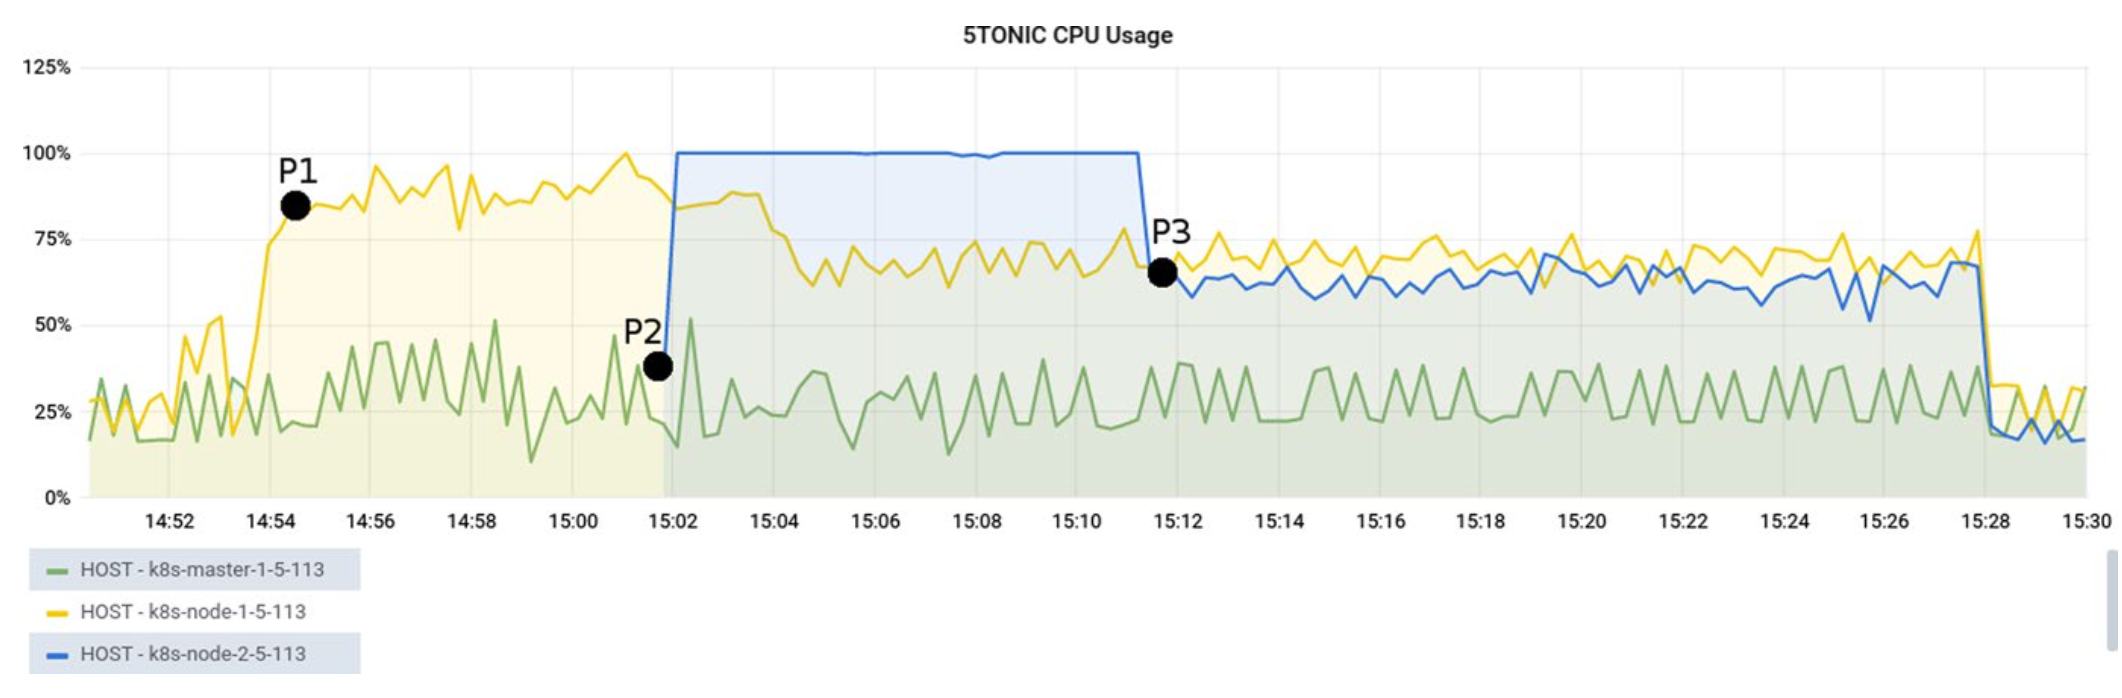
\includegraphics[width=0.8\linewidth]{figs/SEA_Plot_IoT.png}}
                \caption{PoC IoT}
            \end{figure}            
        \end{column}
    \end{columns}
\end{frame}

\begin{frame}{Alocação de Recursos em Redes IoT Multifuncionais\footcite{Silva2024}}
    \begin{figure}
        \centering
        \subfloat{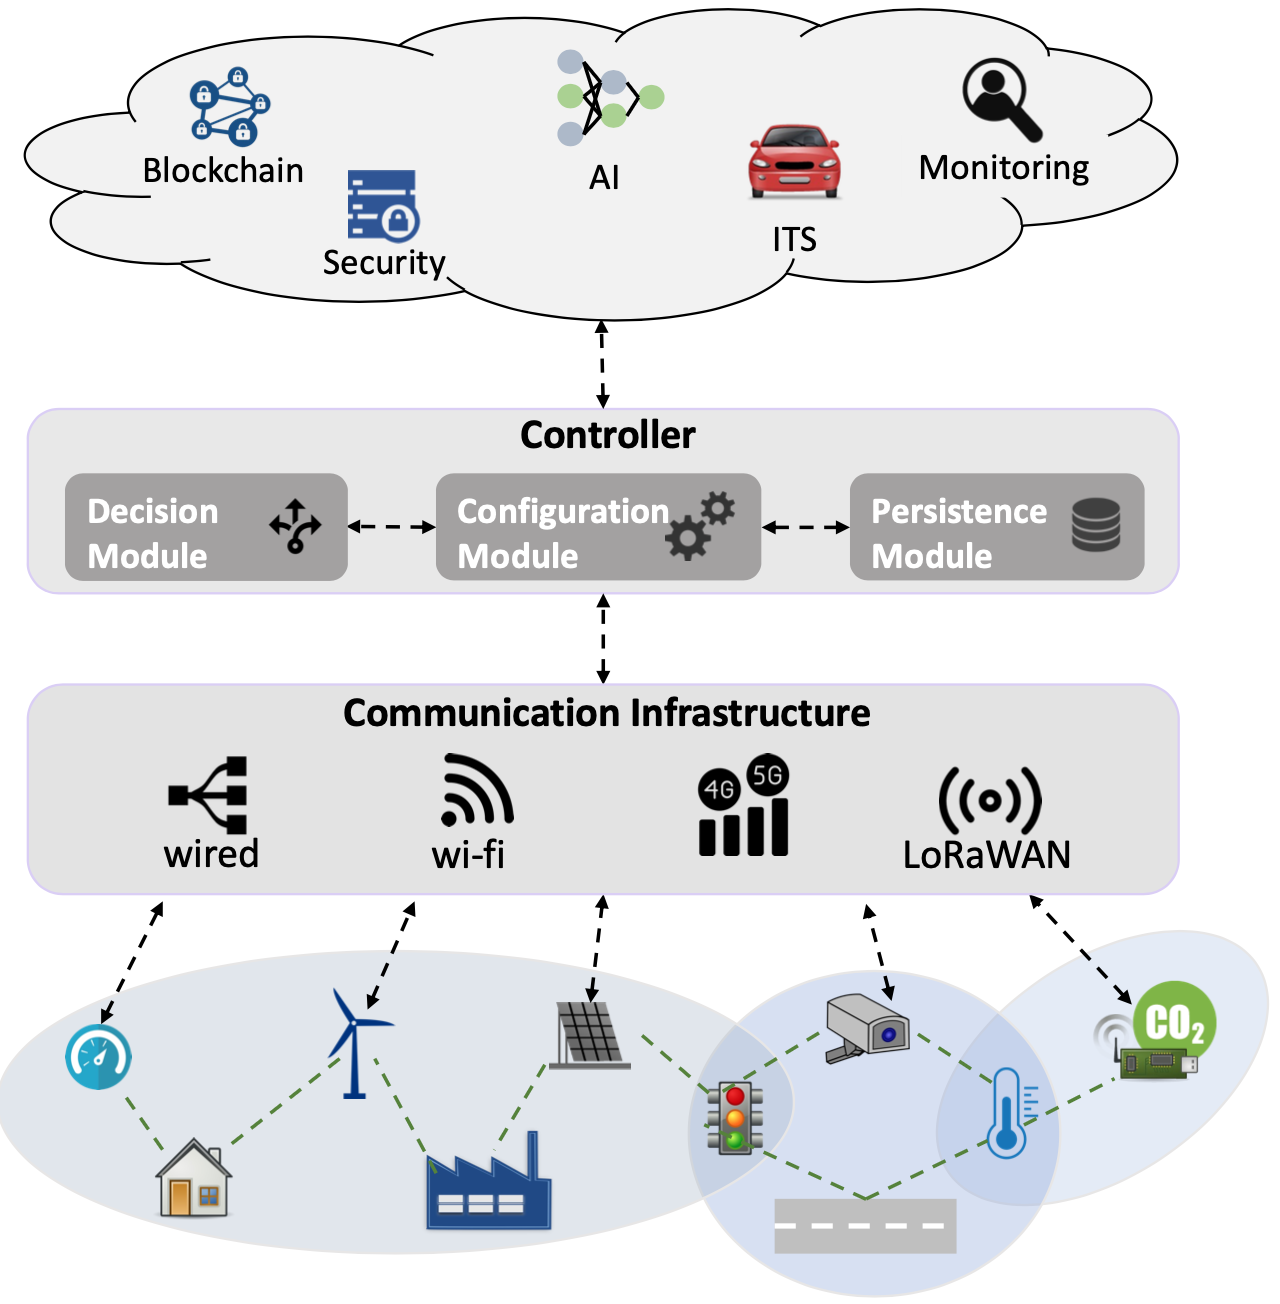
\includegraphics[width=0.5\linewidth]{figs/POSITRON_cenario.png}}
        \hspace{0.5cm}
        \subfloat{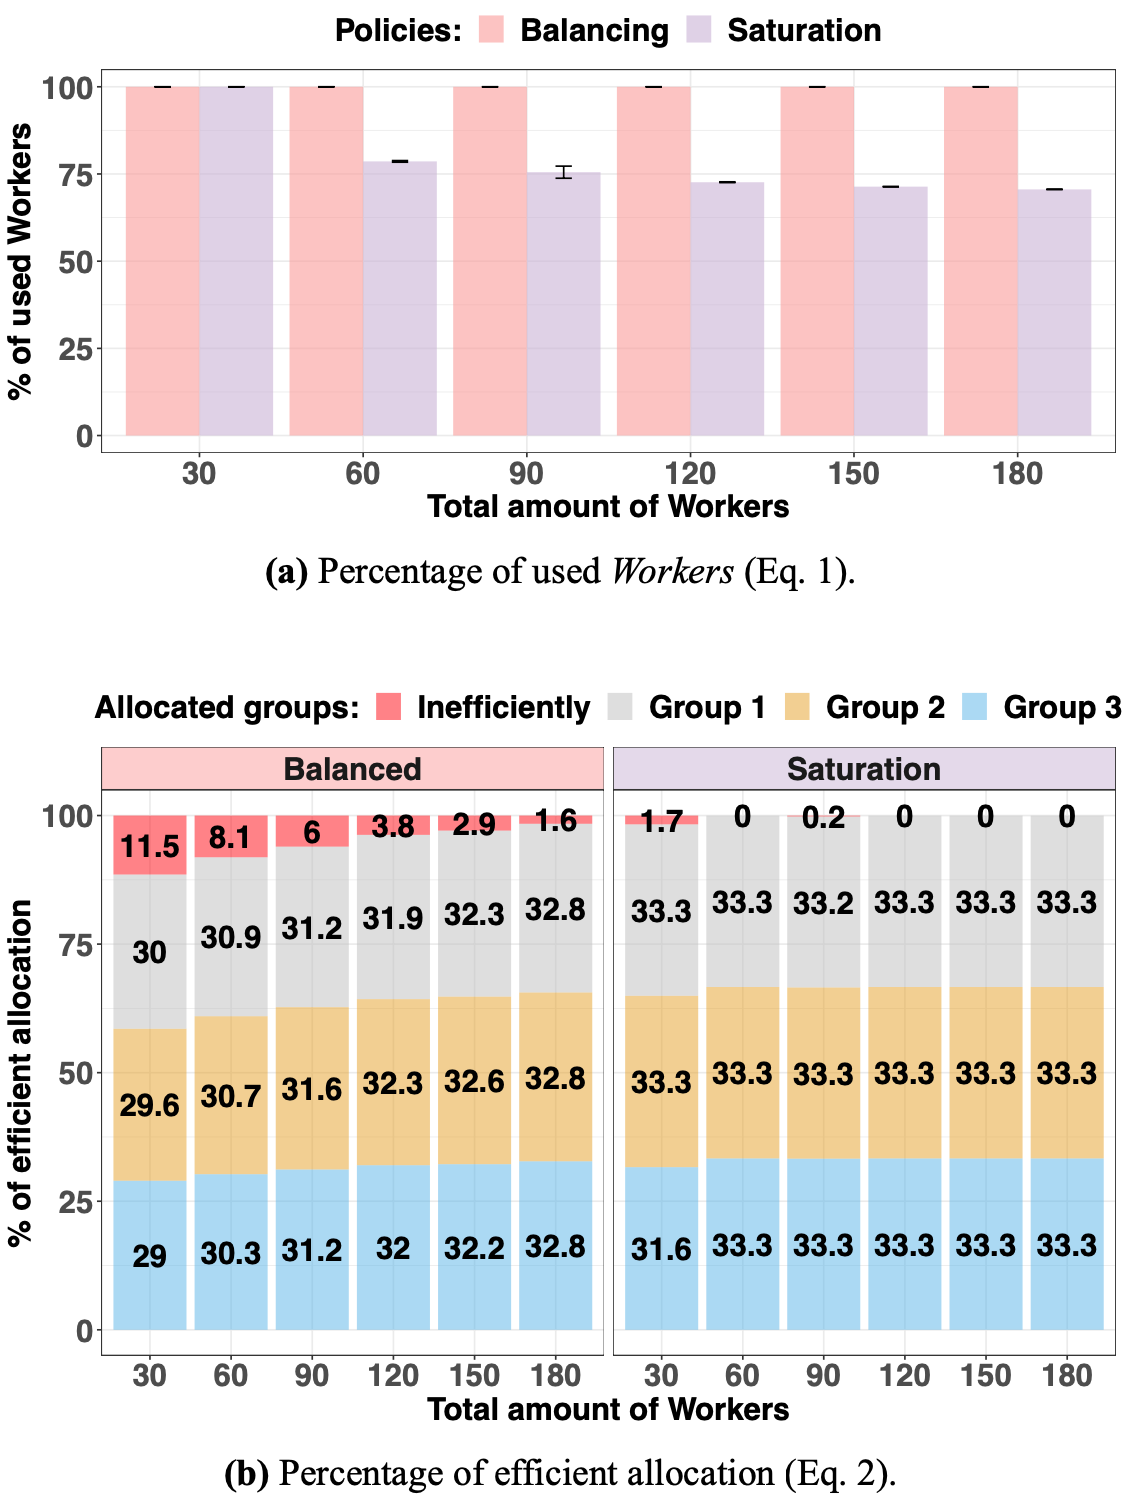
\includegraphics[width=0.4\linewidth]{figs/POSITRON_resultado.png}}
        \caption{Políticas de gerenciamento em redes IoT multifuncionais}
        \label{fig:enter-label}
    \end{figure}
\end{frame}

\begin{frame}{Transmissão de Vídeo em Tempo Real via Rede 5G Privada}
    \begin{columns}
        \begin{column}{0.45\textwidth}
            \begin{itemize}
                \item Implementar ambiente de \textit{testbed} que possibilite experimentação da aplicação de vídeo
                \item Investigar influência da rede de transporte no desempenho das aplicações
                \item Avaliar estratégias para aumento de desempenho na transmissão de vídeo em redes 5G privadas
            \end{itemize}
        \end{column}
        \begin{column}{0.55\textwidth}
            \begin{figure}[htb]
                \centering
                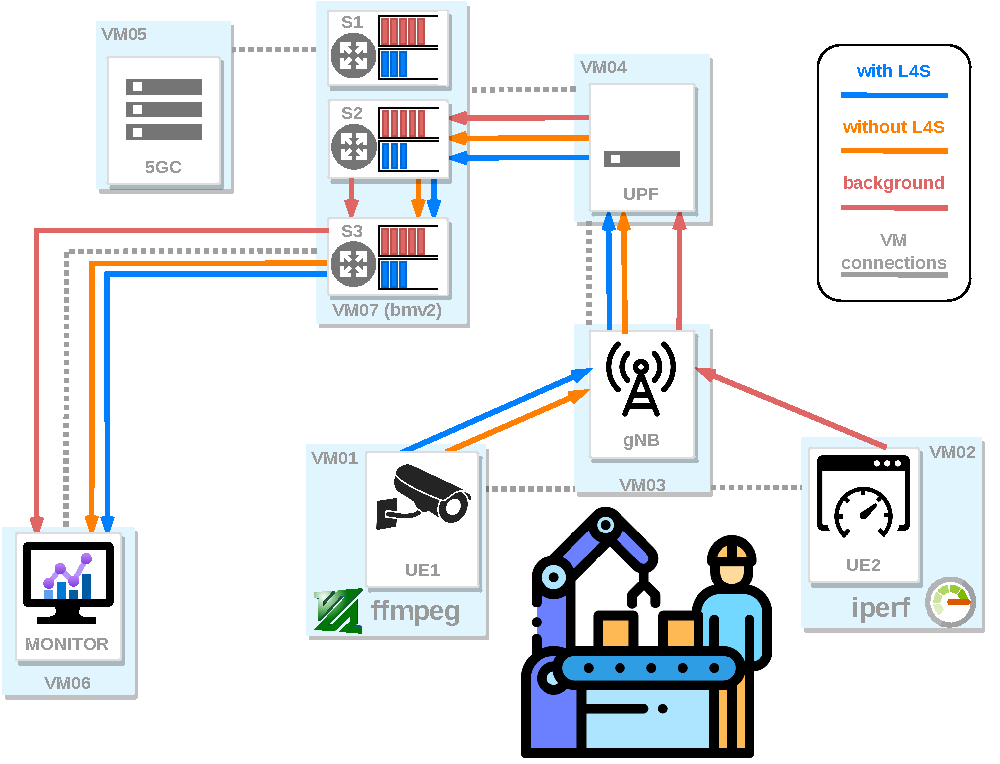
\includegraphics[width=\textwidth]{figs/testbed_5G_privado.pdf}
                \caption{\textit{Testbed} de software com implementação \textit{open source} da rede 5G (autoria própria)}
                \label{fig:setup}
            \end{figure} 
        \end{column}
    \end{columns}
\end{frame}